\section{Dämpfung, Verstärkung, Dezibel}

Hinweis: Neben Dezibel gibt es ein weiteres Dämpfungs-/ bzw. Verstärkungsmass: Neper $\neper$
Auf dieses Mass wird allerdings nicht genauer eingegangen. \textrightarrow\ Skript: S.207


\subsection{Dämpfungsfaktor \texorpdfstring{$D$}{D}}{206}

Das Verhältnis zwischen Eingangs- und Ausgangssignal wird als Dämpfungsfaktor $D$ bezeichnet

\begin{minipage}[c]{0.3\columnwidth}
    $$ \boxed{ D_{P} = \frac{P_{1}}{P_{2}} } $$
\end{minipage}
\hfill
\begin{minipage}[c]{0.3\columnwidth}
    $$ \boxed{ D_{U} = \frac{U_{1}}{U_{2}} } $$
\end{minipage}
\hfill
\begin{minipage}[c]{0.3\columnwidth}
    $$ \boxed{ D_{I} = \frac{I_{1}}{I_{2}} } $$
\end{minipage}

Die Indizes $U$, $P$, $I$ stehen für die \textbf{Effektivwerte} von Spannung, Leistung und Strom.


\subsection{Dämpfungsmass \texorpdfstring{$a$}{a} in Dezibel}{206}

Durch \textbf{logarithmieren} des Dämpfungsfaktors $D$ erhält man das Dämpfungsmass $a$

\begin{minipage}[c]{0.3\columnwidth}
    $$ \boxed{ a_{P} =  10 \cdot \log_{10} \Big( \frac{P_{1}}{P_{2}} \Big) } $$
\end{minipage}
\hfill
\begin{minipage}[c]{0.3\columnwidth}
    $$ \boxed{ a_{U} = 20 \cdot \log_{10} \Big( \frac{U_{1}}{U_{2}} \Big) } $$
\end{minipage}
\hfill
\begin{minipage}[c]{0.3\columnwidth}
    $$ \boxed{ a_{I} = 20 \cdot \log_{10} \Big( \frac{I_{1}}{I_{2}} \Big) } $$
\end{minipage}


\subsubsection{Umrechnung Verstärkungsfaktor -- Dezibel}

$$ \boxed{ \deci\bel = 10 \cdot \log_{10} (v) \, \Leftrightarrow \, v = 10^{\frac{\deci\bel}{10}} } $$


\subsection{Rechenregeln mit Dezibel}

\begin{itemize}
    \item Faktoren multiplizieren \textrightarrow\ Dezibel-Werte addieren
    \item Faktoren dividieren \textrightarrow\ Dezibel-Werte subtrahieren
\end{itemize}


\subsection{Spannungsverstärkungsfaktor}{209}

Hält man sich strikt an die Definition des Verstärkungsfaktors bzw. die Definition der Dezibel, so würde man für Dämpfungen positive
Dezibel-Werte erhalten und für Verstärkungen entspreched negative Dezibel-Werte. Dies ist gegen die Intuition des Ingenieurs. \\
Somit wurde der \textbf{Spannungsverstärkungsfaktor} $\bm{T_{U}}$ definiert. Analog zum Dämpfungsmass $a$ wird ein 
\textbf{Verstärkungsmass} $\bm{g_{U}}$ definiert.

\begin{minipage}[c]{0.48\columnwidth}
    $$ \boxed{ T_U = \frac{U_2}{U_1} } $$
\end{minipage}
\hfill
\begin{minipage}[c]{0.48\columnwidth}
    $$ \boxed{ g_U = 20 \cdot \log_{10} \Big( \frac{U_2}{U_1} \Big) } $$
\end{minipage}


Aus dieser Definition folgt für die Dezibel-Werte:

\begin{itemize}
    \item \textbf{Verstärkung: } ($U_2 > U_1$) \textrightarrow\ positive Dezibel-Zahl
    \item \textbf{Dämpfung: } ($U_2 < U_1$) \textrightarrow\ negative Dezibel-Zahl
\end{itemize}


\example{Kaskadiertes System}{209}

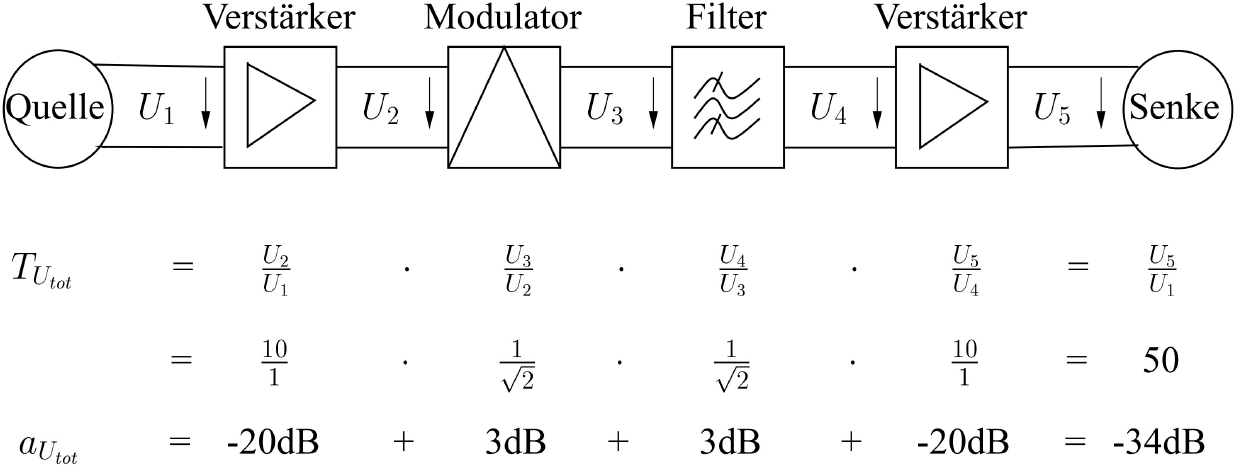
\includegraphics[width=0.9\columnwidth]{images/kaskadierung_verstaerkung_daempfung.png}

Formuliert mit dem Verstärkungsmass $g$ ergeben sich umgekehrte Vorzeichen:
$$ g_{U_{\rm tot}} \quad = \quad - 20 \, \deci\bel \quad  + \quad 3 \, \deci\bel \quad + 
    \quad 3 \, \deci\bel \quad - \quad 20 \, \deci\bel \quad = \quad -34 \, \deci\bel $$


\subsection{Umrechnungs-Tabelle Dezibel -- Faktor}

\textbf{Vorgehen:} Gesuchten $\deci\bel$-Wert als Summe / Differenz von bekannten Werten darstellen\\
\textrightarrow\ Summanden in Faktoren 'transferieren' und multiplizieren / dividieren \medskip

\textbf{Vorgehen:} Gesuchten Faktor als Produkt / Quotent von bekannten Werten darstellen\\
\textrightarrow\ Faktoren in Summanden 'transferieren' und addieren / subtrahieren \medskip


\begin{ctabular}{l l}
    \toprule
    \textbf{Dezibel}        & \textbf{Faktor} \\
    \midrule
    $20 = 10 + 10$          & $100 = 10 \cdot 10$ \\ 
    $12$                    & $16 = 2 \cdot 2 \cdot 2 \cdot 2$ \\
    $\cor{10}$              & $\cor{10}$ \\
    $9 = 3 + 3 + 3$         & $8 = 2 \cdot 2 \cdot 2$ \\
    $8 = 5 - 3$             & $6.4 = 3.2 \cdot 2$ \\
    $7 = 10 -3$             & $5 = \frac{10}{2}$ \\
    $6 = 3 + 3$             & $4 = 2 \cdot 2$ \\
    $5 = 15 - 10$           & $3.2 = \frac{32}{10\mathstrut} \approx \sqrt{10}$ \\
    $4 = 10 - 6 = 10 - 3-3$ & $2.5 = \frac{10\mathstrut}{2 \cdot 2}$ \\
    $\cor{3}$               & $\cor{2}$ \\
    $2= 12-10= 5-3$         & $1.6 = \frac{16}{10}$ \\
    $1 = 10 - 3 - 3 - 3$    & $1.25 = \frac{10}{2\cdot 2 \cdot 2} = \frac{5}{4}$ \\
    $\cor{0}$               & $\cor{1}$ \\
    $-1$                    & $0.8 = \frac{4}{5}$ \\
    \bottomrule
\end{ctabular}


\subsection{Relativer und Absoluter Pegel}{210}

Bei den bisher ausgeführten Pegeln handelt es sich um \textbf{relative Pegel}. Im Gegensatz dazu beziehen sich
\textbf{absolute Pegelangaben} immer auf eine Referenzgrösser (erzeugt von einem Normengenerator, siehe Skript). 

\renewcommand{\arraystretch}{1.7}
\begin{tabular}{c c c}
    ${(L_{U})}_{\rm rel} = 20 \cdot \log_{10} \left\lgroup \frac{U_2}{U_1} \right\rgroup$ & &
    ${(L_{U})}_{\rm abs} = 20 \cdot \log_{10} \left\lgroup \frac{U_2}{774.6 \, \milli\volt} \right\rgroup$ \\
    
    ${(L_{I})}_{\rm rel} = 20 \cdot \log_{10} \left\lgroup \frac{I_2}{I_1} \right\rgroup$ & &
    ${(L_{I})}_{\rm abs} = 20 \cdot \log_{10} \left\lgroup \frac{I_2}{1.291 \, \milli\ampere} \right\rgroup$ \\
    
    ${(L_{P})}_{\rm rel} = 10 \cdot \log_{10} \left\lgroup \frac{P_2}{P_1} \right\rgroup$ & &
    ${(L_{P})}_{\rm abs} = 10 \cdot \log_{10} \left\lgroup \frac{P_2}{1 \, \milli\watt} \right\rgroup$ \\
\end{tabular}
\renewcommand{\arraystretch}{1}


\subsubsection{Kennzeichnung absoluter Pegel}

\begin{center}
    \begin{tabular}{ll}
        \textbf{Notation}       & \textbf{Bezugsgrösse} \\
        $\deci\bel\watt$        & $1 \, \watt$          \\
        $\deci\bel\volt$        & $1 \, \volt$          \\
    \end{tabular}\hspace{5mm}
    \begin{tabular}{ll}
        \textbf{Notation}       & \textbf{Bezugsgrösse} \\
        $\deci\bel\milli$       & $1 \, \milli \watt$ \\
        $\deci\bel\micro\volt$  & $1 \, \micro \watt$ 
    \end{tabular}
\end{center}
